\section{Patrones Arquitectónicos}
	\noindent Para complementar el diseño basado en Microservicios y la Arquitectura Orientada a Eventos (EDA), se proponen los siguientes patrones arquitectónicos. Cada uno resuelve necesidades específicas relacionadas con escalabilidad, comunicación entre servicios, separación de responsabilidades y resiliencia.
	
	\subsection*{1. API Gateway}
		\begin{itemize}
			\item \textbf{Descripción:} Patrón que establece una única puerta de entrada para acceder a múltiples microservicios.  
			\item \textbf{Descripción:} Patrón que establece una única puerta de entrada para acceder a múltiples microservicios.  
			\item \textbf{Aplicación en Casa Fácil:} El API Gateway (ej. Nginx o Kong) será el primer punto de contacto para el cliente. Centraliza la gestión de autenticación, autorización, enrutamiento de solicitudes y limitación de tráfico.  
			\item 	\textbf{Ventajas:}
			\begin{itemize}
				\item Oculta la complejidad interna del sistema.
				\item Reduce el acoplamiento entre cliente y servicios individuales.
				\item Permite control centralizado de seguridad y monitoreo.
			\end{itemize}
		\end{itemize}
		\begin{center}
			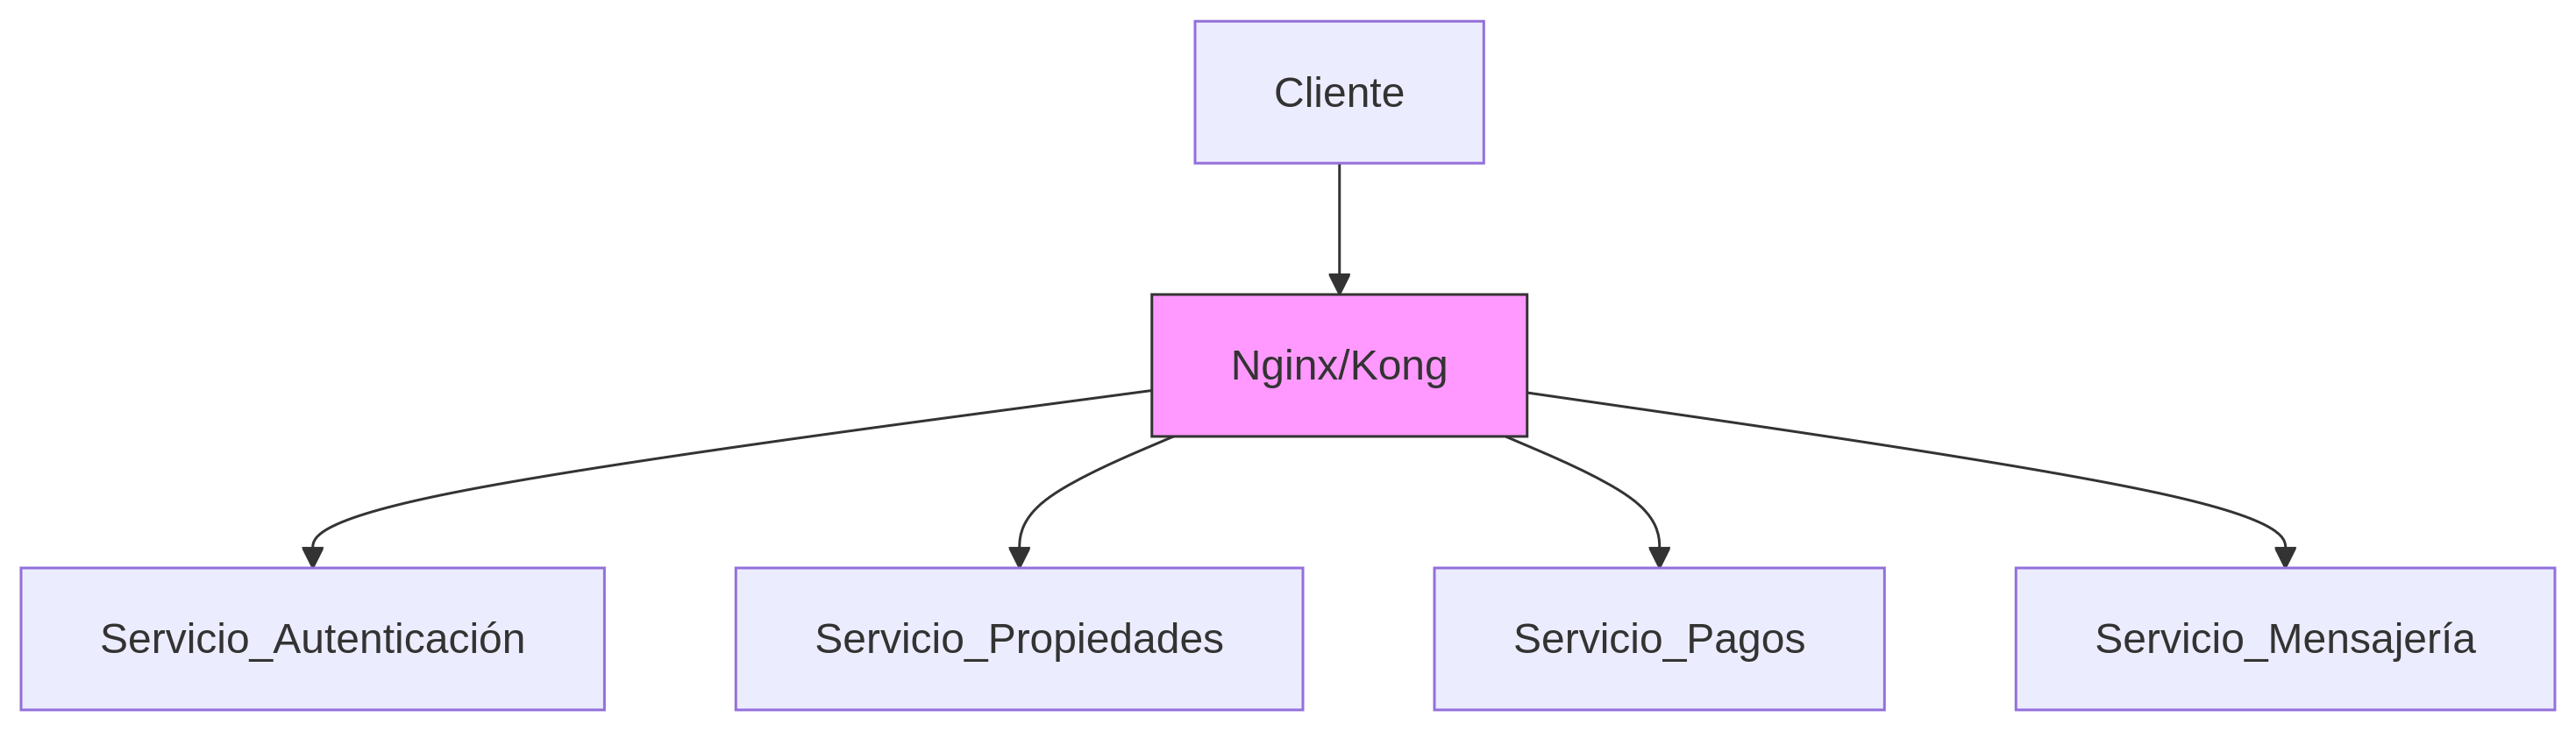
\includegraphics[width=\linewidth]{figures/patterns/APIG.png}
			\captionof{figure}{Componentes API Gateway.}
			\label{fig:img2}
		\end{center}
	
	\subsection*{2. CQRS (Command Query Responsibility Segregation)}
		\begin{itemize}
			\item \textbf{Descripción:} Separa las operaciones de lectura (consultas) de las de escritura (comandos), permitiendo optimizar y escalar cada una por separado.  
			\item \textbf{Aplicación en Casa Fácil:} En funcionalidades como gestión de reservas o propiedades, el modelo de lectura puede ser distinto y más optimizado que el modelo de escritura, por ejemplo, consultas masivas de propiedades vs. edición de una publicación.  
			\item \textbf{Ventajas:}
			\begin{itemize}
				\item Mejora el rendimiento y escalabilidad.
				\item Facilita el uso de diferentes tecnologías para leer y escribir.
				\item Ideal para sistemas con alto volumen de datos y lógica compleja.
			\end{itemize}
		\end{itemize}
		\begin{center}
			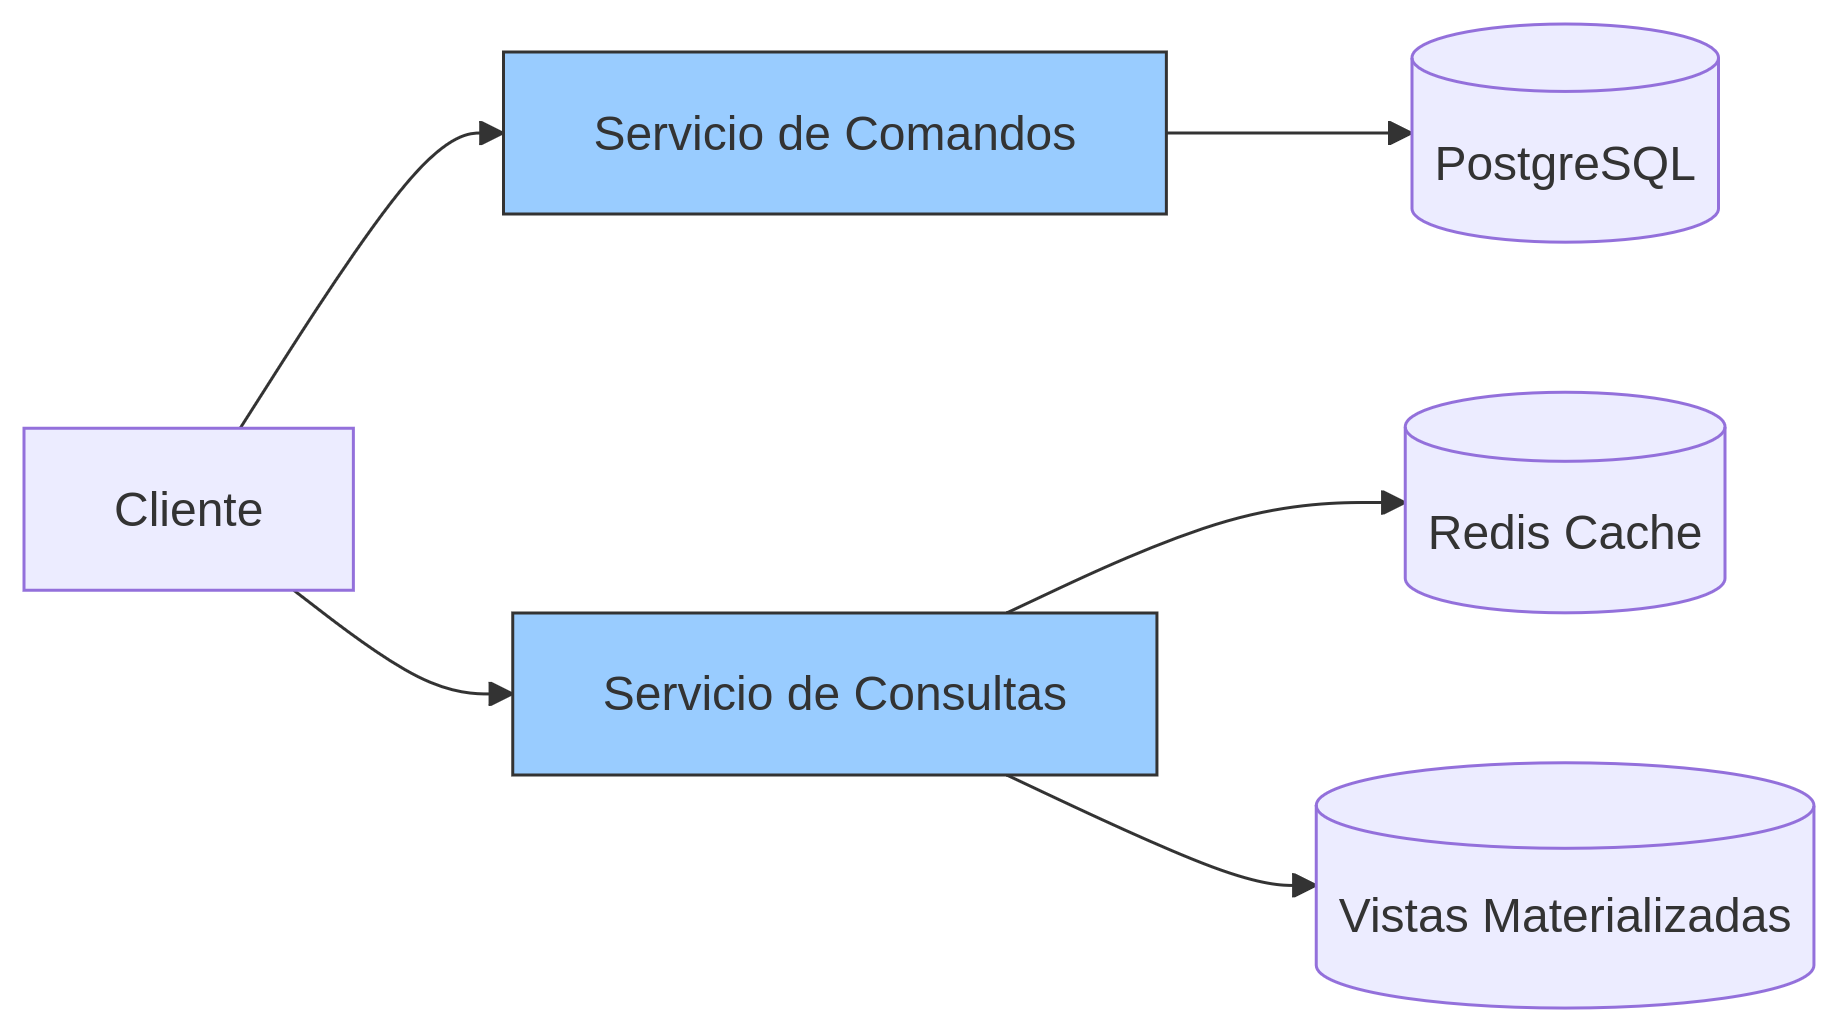
\includegraphics[width=\linewidth]{figures/patterns/CQRS.png}
			\captionof{figure}{Componentes CQRS.}
			\label{fig:img3}
		\end{center}
	
	\subsection*{3. Event Sourcing}
		\begin{itemize}
			\item \textbf{Descripción:} En lugar de almacenar el estado actual de una entidad, se almacena una secuencia de eventos que modificaron su estado.  
			\item \textbf{Aplicación en Casa Fácil:} Para gestionar el historial de reservas, cambios de disponibilidad o pagos, se puede almacenar cada evento como "propiedad reservada", "pago confirmado".  
			\item 	\textbf{Ventajas:}
			\begin{itemize}
				\item Trazabilidad completa de acciones pasadas.
				\item Reversión de cambios y auditoría sencilla.
				\item Se complementa naturalmente con EDA.
			\end{itemize}
		\end{itemize}
		\begin{center}
			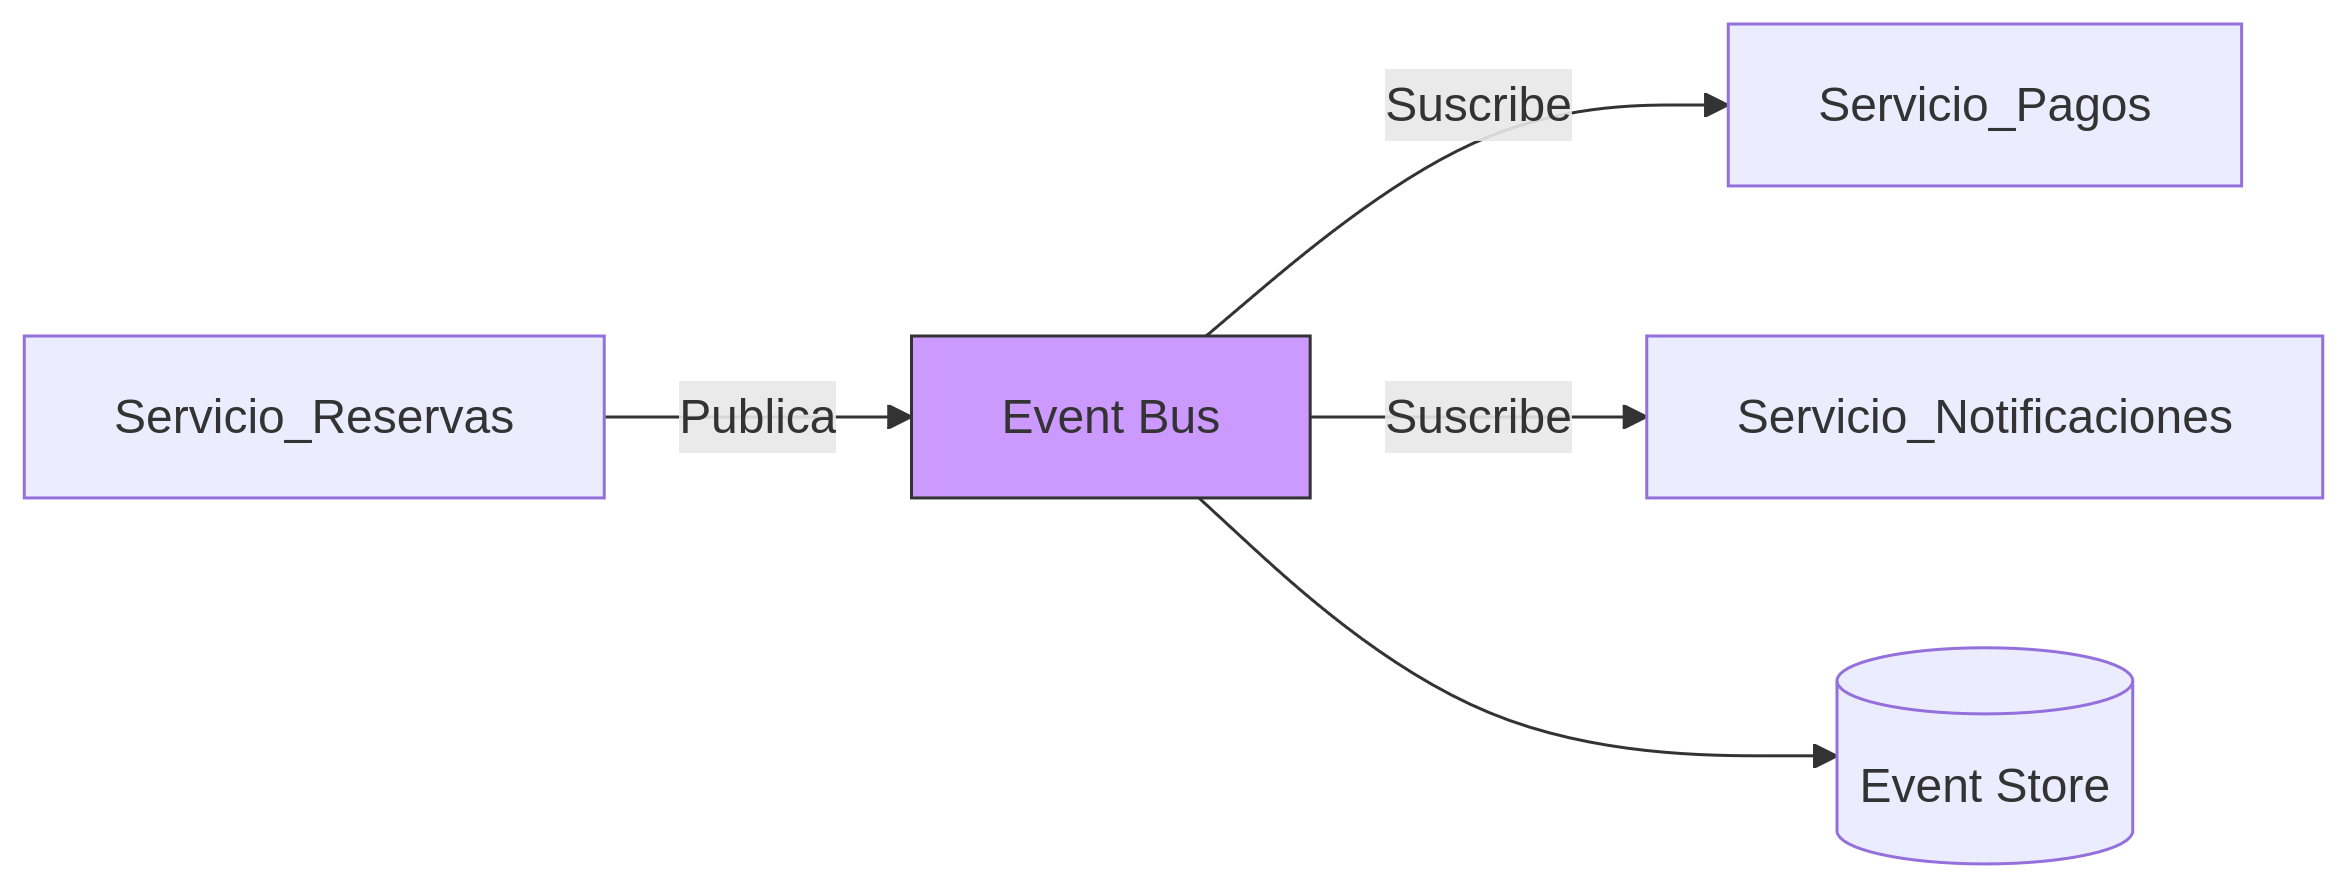
\includegraphics[width=\linewidth]{figures/patterns/EVENT.png}
			\captionof{figure}{Componentes Event Sourcing.}
			\label{fig:img4}
		\end{center}
		
	\subsection*{4. Service Registry \& Discovery}
		\begin{itemize}
			\item \textbf{Descripción:} Permite que los microservicios se registren en un directorio común para ser descubiertos dinámicamente.  
			\item \textbf{Aplicación en Casa Fácil:} En entornos con múltiples servicios desplegados dinámicamente (como en contenedores Docker), el registro facilita la comunicación entre servicios sin direcciones IP fijas.  
			\item 	\textbf{Ventajas:}
			\begin{itemize}
				\item Reducción de la configuración manual.
				\item Mejor soporte para escalado automático.
				\item Necesario para balanceo de carga dinámico.
			\end{itemize}
		\end{itemize}
		\begin{center}
			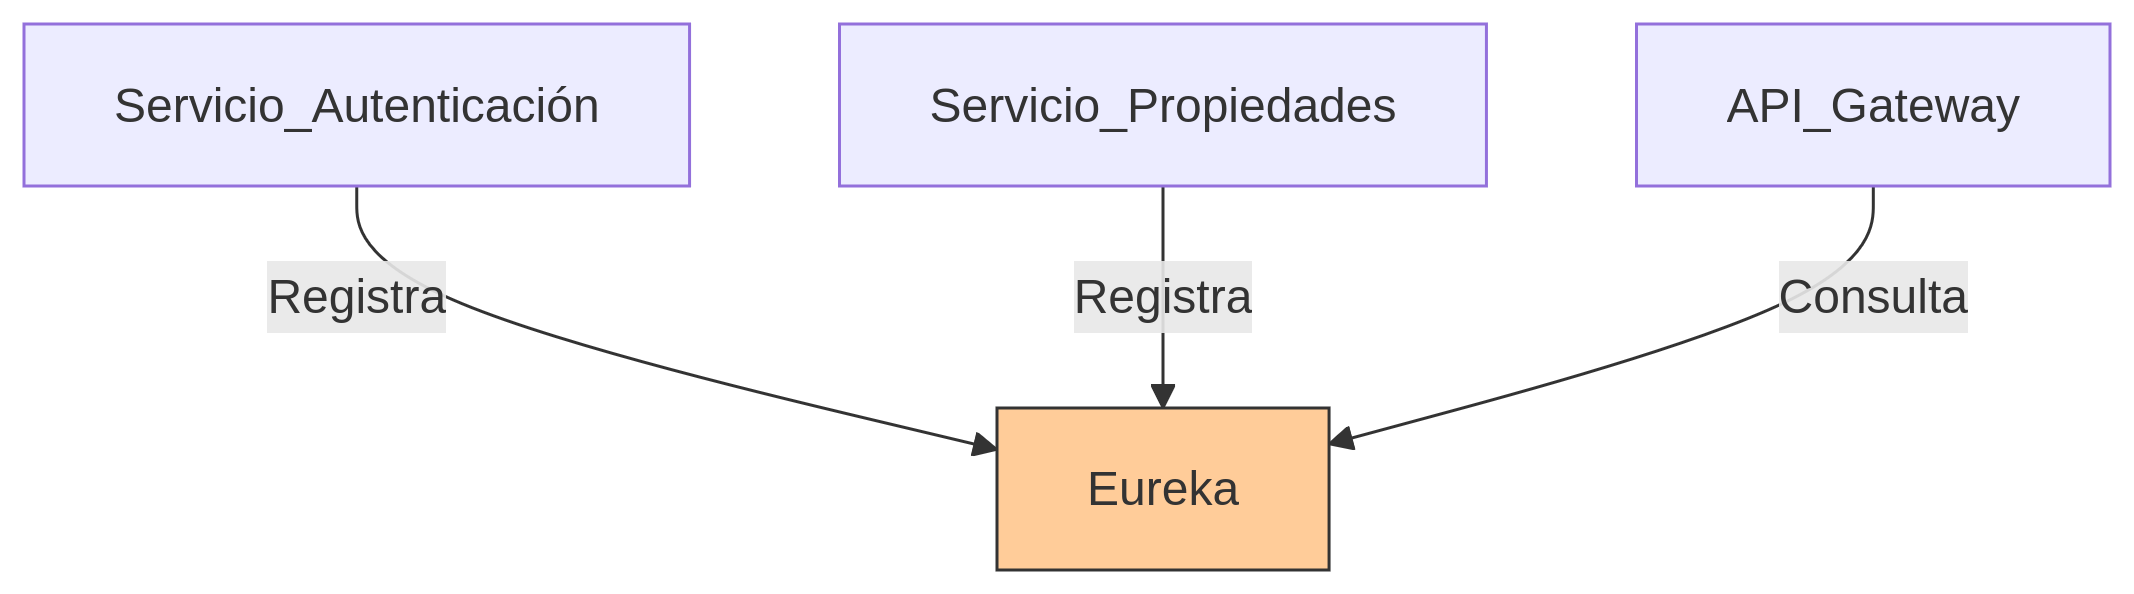
\includegraphics[width=\linewidth]{figures/patterns/SERVICE_R_D.png}
			\captionof{figure}{Componentes Service Registry \& Discovery.}
			\label{fig:img5}
		\end{center}
	
	\subsection*{5. Backend for Frontend (BFF)}
		\begin{itemize}
			\item \textbf{Descripción:} Crea una capa intermedia específica para cada tipo de cliente (web, móvil, etc.), adaptando las respuestas del backend a sus necesidades.  
			\item \textbf{Aplicación en Casa Fácil:} La versión móvil puede tener un BFF que priorice velocidad y respuesta ligera, mientras que la web puede entregar más datos.  
			\item 	\textbf{Ventajas:}
			\begin{itemize}
				\item Reduce carga y complejidad en el frontend.
				\item Mejora la experiencia de usuario según el dispositivo.
				\item Facilita la evolución independiente de interfaces.
			\end{itemize}
		\end{itemize}
		\begin{center}
			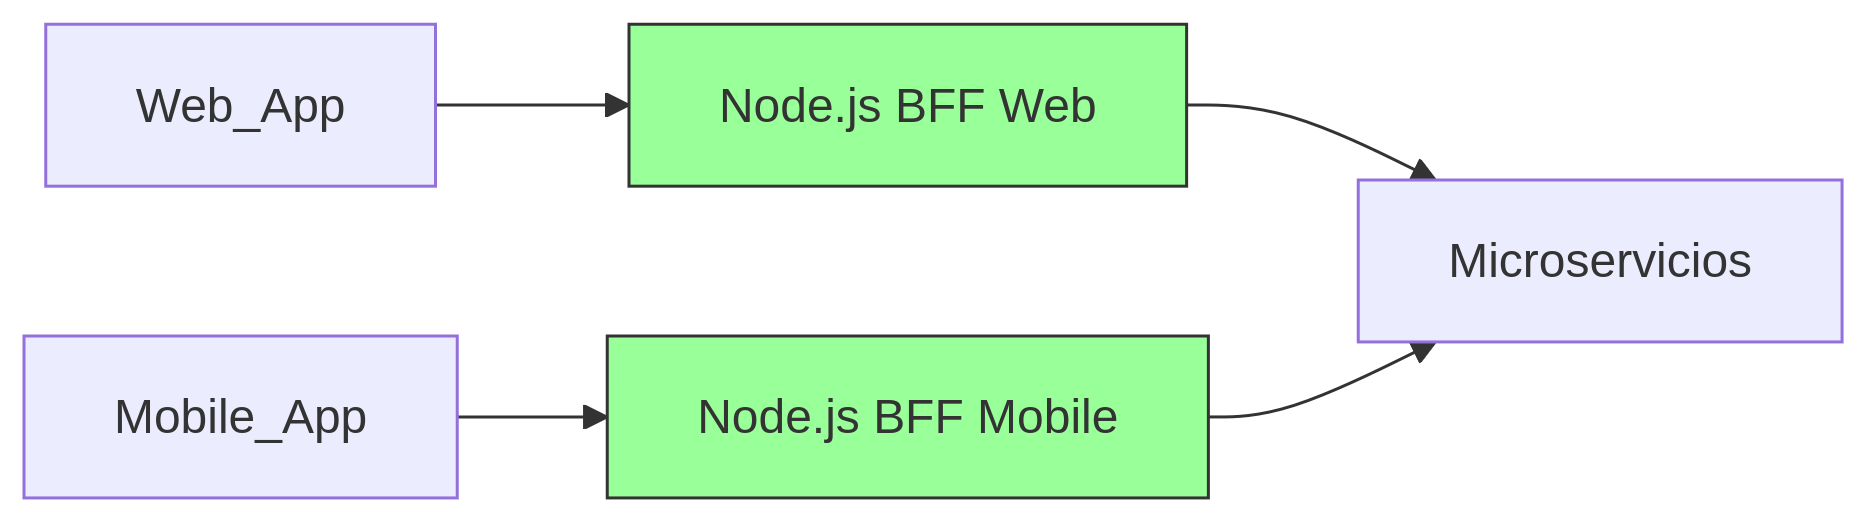
\includegraphics[width=\linewidth]{figures/patterns/BACKEND.png}
			\captionof{figure}{Componentes Backend for Frontend.}
			\label{fig:img6}
		\end{center}
	
	\subsection*{6. Saga}
		\begin{itemize}
			\item \textbf{Descripción:} Coordina transacciones distribuidas entre múltiples servicios, garantizando consistencia eventual a través de una serie de pasos y compensaciones si algo falla.  
			\item \textbf{Aplicación en Casa Fácil:} Una reserva de propiedad puede requerir verificar disponibilidad, generar pago y enviar notificación. Si el pago falla, debe deshacerse todo.  
			\item \textbf{Ventajas:}
			\begin{itemize}
				\item Maneja flujos de negocio complejos sin transacciones bloqueantes.
				\item Aumenta la confiabilidad en flujos asincrónicos.
				\item Escalable y desacoplado.
			\end{itemize}
		\end{itemize}
		\begin{center}
			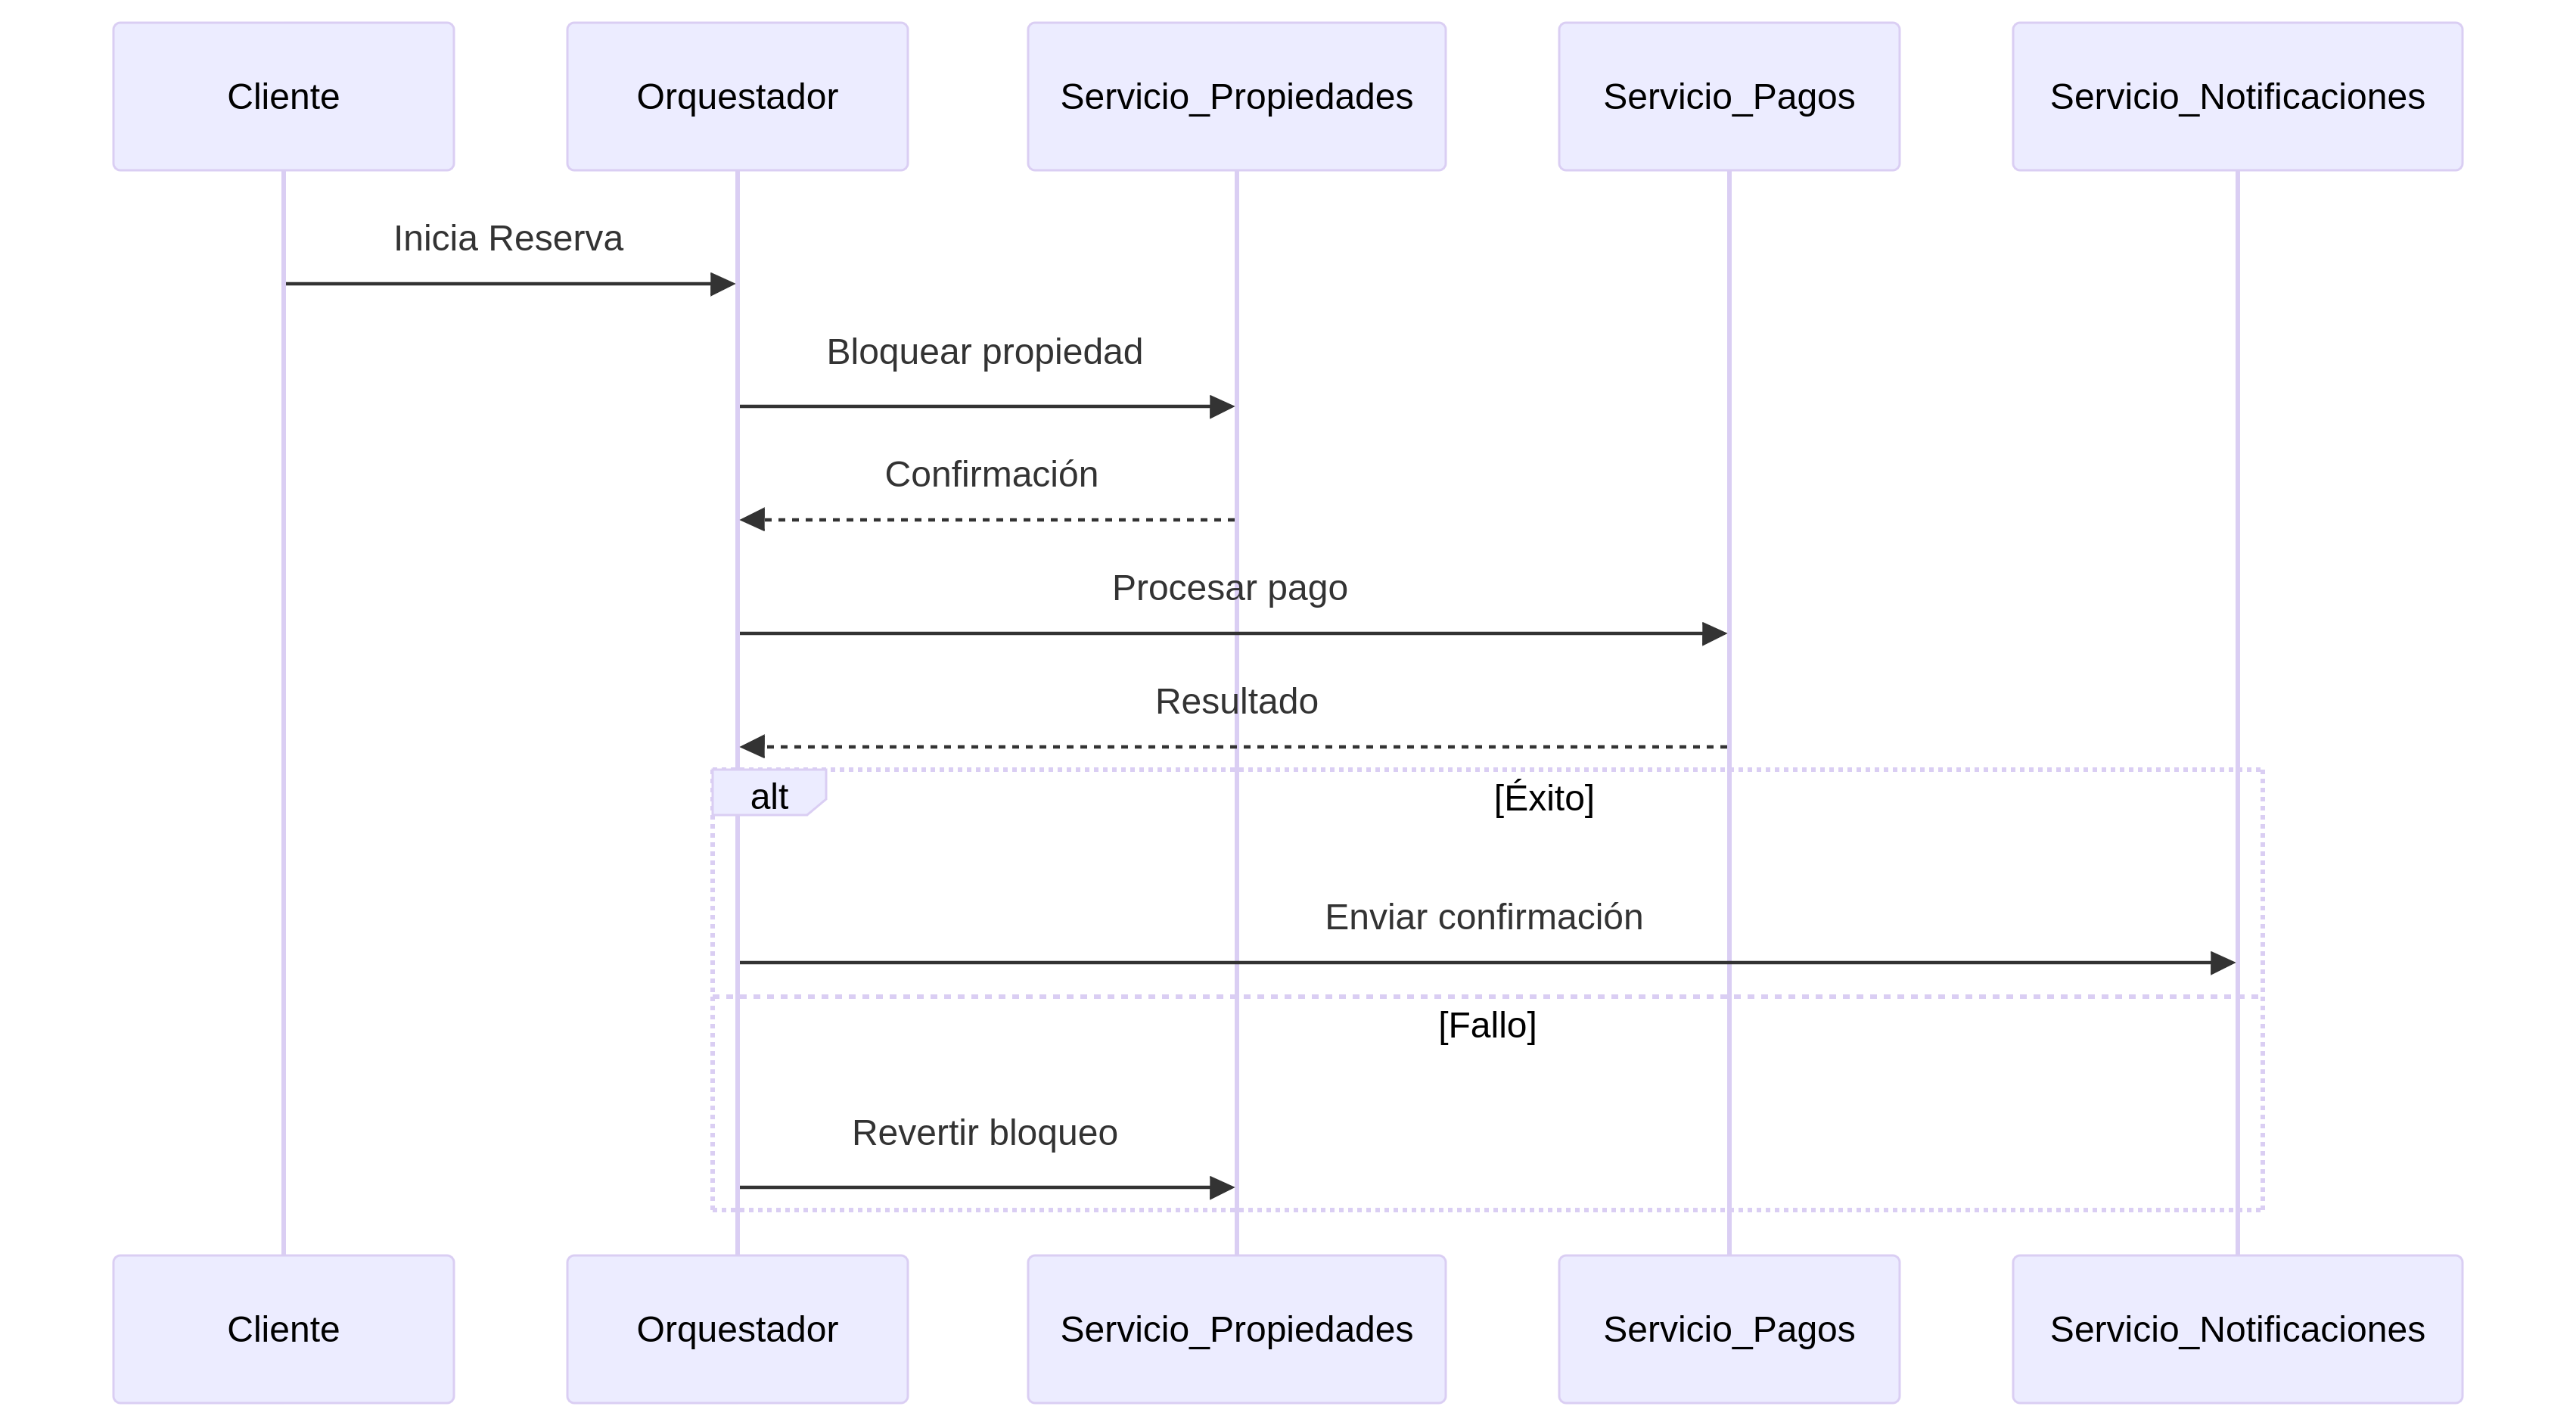
\includegraphics[width=\linewidth]{figures/patterns/SAGA.png}
			\captionof{figure}{Componentes Saga.}
			\label{fig:img7}
		\end{center}
	
	\subsection*{7. Strangler Fig}
		\begin{itemize}
			\item \textbf{Descripción:} Permite reemplazar gradualmente un sistema monolítico por microservicios. Se encapsula el sistema antiguo y se introducen nuevos componentes uno por uno.  
			\item \textbf{Aplicación en Casa Fácil:} Si partes del sistema comienzan siendo monolíticas (como reservas o pagos), pueden migrarse paulatinamente sin interrumpir la operación.  
			\item \textbf{Ventajas:}
			\begin{itemize}
				\item Reducción del riesgo en la migración.
				\item Permite evolución controlada del sistema.
				\item Compatible con despliegue incremental.
			\end{itemize}
		\end{itemize}
		\begin{center}
			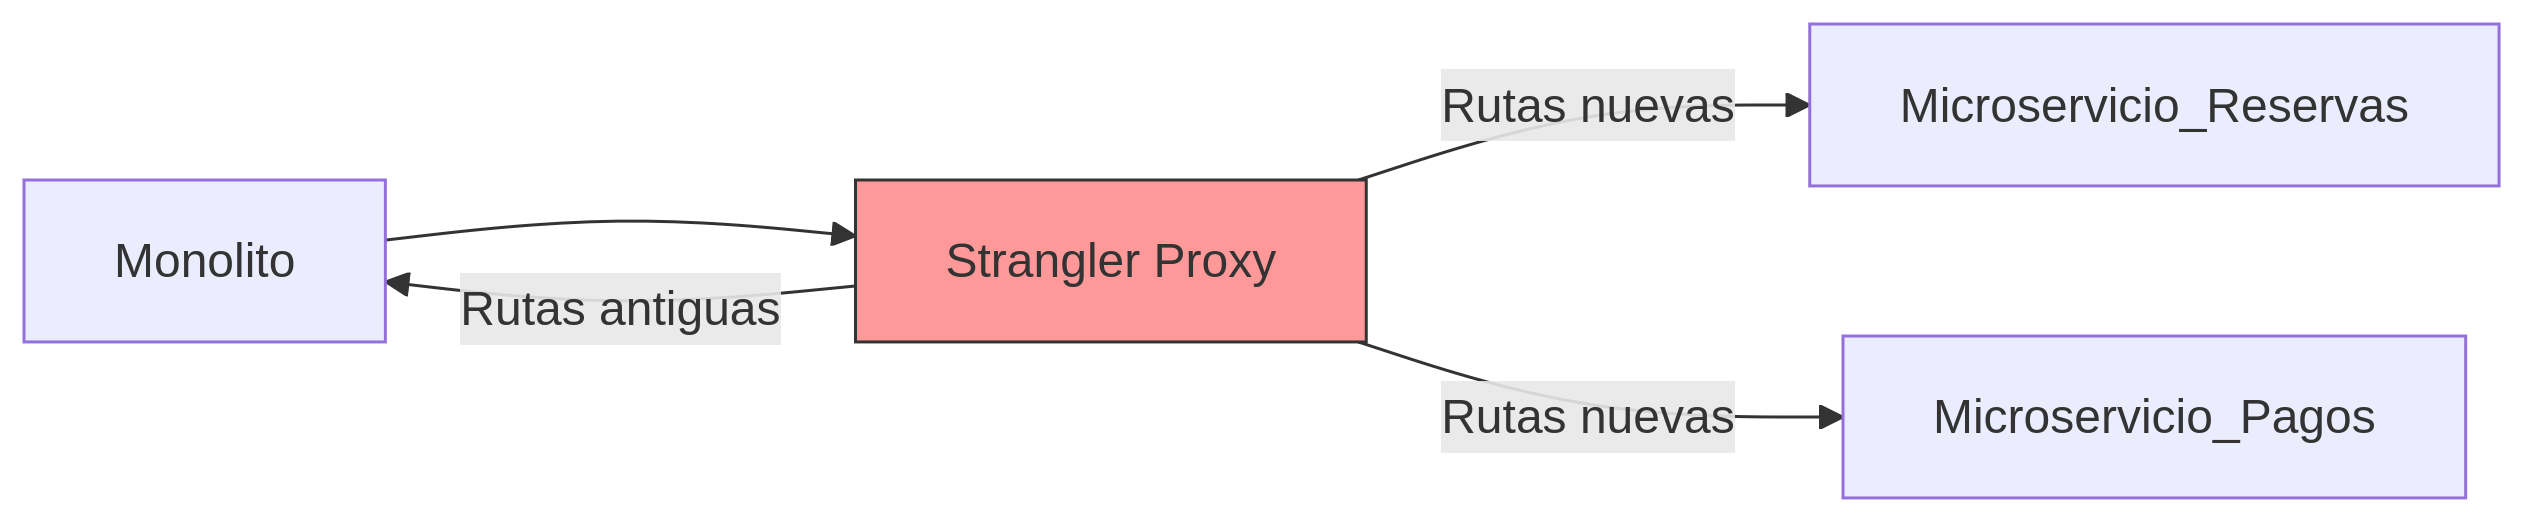
\includegraphics[width=\linewidth]{figures/patterns/STRANGLER.png}
			\captionof{figure}{Componentes Strangler Fig.}
			\label{fig:img8}
		\end{center}